\section{Исследовательский раздел \hfill}
\vspace{\baselineskip}

В данном разделе приводятся результаты опроса респондентов и примеры работы программы.

\vspace{\baselineskip}
\subsection{Опрос респондентов} 
\vspace{\baselineskip}

В опросе принимали участие следующие студенты:
\begin{enumerate}
    \item Григоренко Е. А. (ИУ7-55Б);
    \item Иванов П. А. (ИУ7-55Б);
    \item Ильин Д. А. (ИУ7-55Б);
    \item Киселева М. С. (ИУ7-56Б);
    \item Саркисян А. А. (ИУ7-55Б).
\end{enumerate}

Результаты опроса приведены в таблице \ref{tabular:asking}, где Б --- близко, С --- средне, Д --- далеко относительно Земли.

\begin{table}[h!]
	\begin{center}
	    \begin{threeparttable}
	    \captionsetup{justification=raggedright, singlelinecheck=off}
	    \caption{\label{tabular:asking} Результаты опроса}
		\begin{tabular}{|c|c|c|c|c|c|c|c|}
			\hline
			Респондент & Меркурий & Венера & Марс & Юпитер & Сатурн & Уран & Нептун \tabularnewline 
                \hline
                1 & С & Б & Б & Д & Д & Д & Д \\
                \hline
                2 & Д & Б & Б & Д & Д & Д & Д \\
			\hline
                3 & С & Б & Б & С & С & Д & Д \\
                \hline
                4 & Д & Б & С & С & С & Д & Д \\
                \hline
                5 & С & Б & Б & С & Д & Д & Д \\
                \hline
		\end{tabular}
		\end{threeparttable}
	\end{center}
\end{table}

Количество людей, выбравших тот или иной вариант для конкретной планеты, представлено в таблице \ref{tabular:pivot}.
\clearpage

\begin{table}[h!]
	\begin{center}
	    \begin{threeparttable}
	    \captionsetup{justification=raggedright, singlelinecheck=off}
	    \caption{\label{tabular:pivot} Сводная таблица}
		\begin{tabular}{|c|c|c|c|c|c|c|c|}
                \hline
                & Меркурий & Венера & Марс & Юпитер & Сатурн & Уран & Нептун \tabularnewline 
                \hline
                Б & 0 & 5 & 4 & 0 & 0 & 0 & 0 \\
                \hline
                С & 3 & 0 & 1 & 3 & 2 & 0 & 0 \\
			\hline
                Д & 2 & 0 & 0 & 2 & 3 & 5 & 5 \\
                \hline
		\end{tabular}
		\end{threeparttable}
	\end{center}
\end{table}

На рисунке \ref{fig:answers} представлены графики функций принадлежности значений переменной термам, описывающим группы значений лингвистической переменной.

\begin{figure}[h!btp]
	\centering
	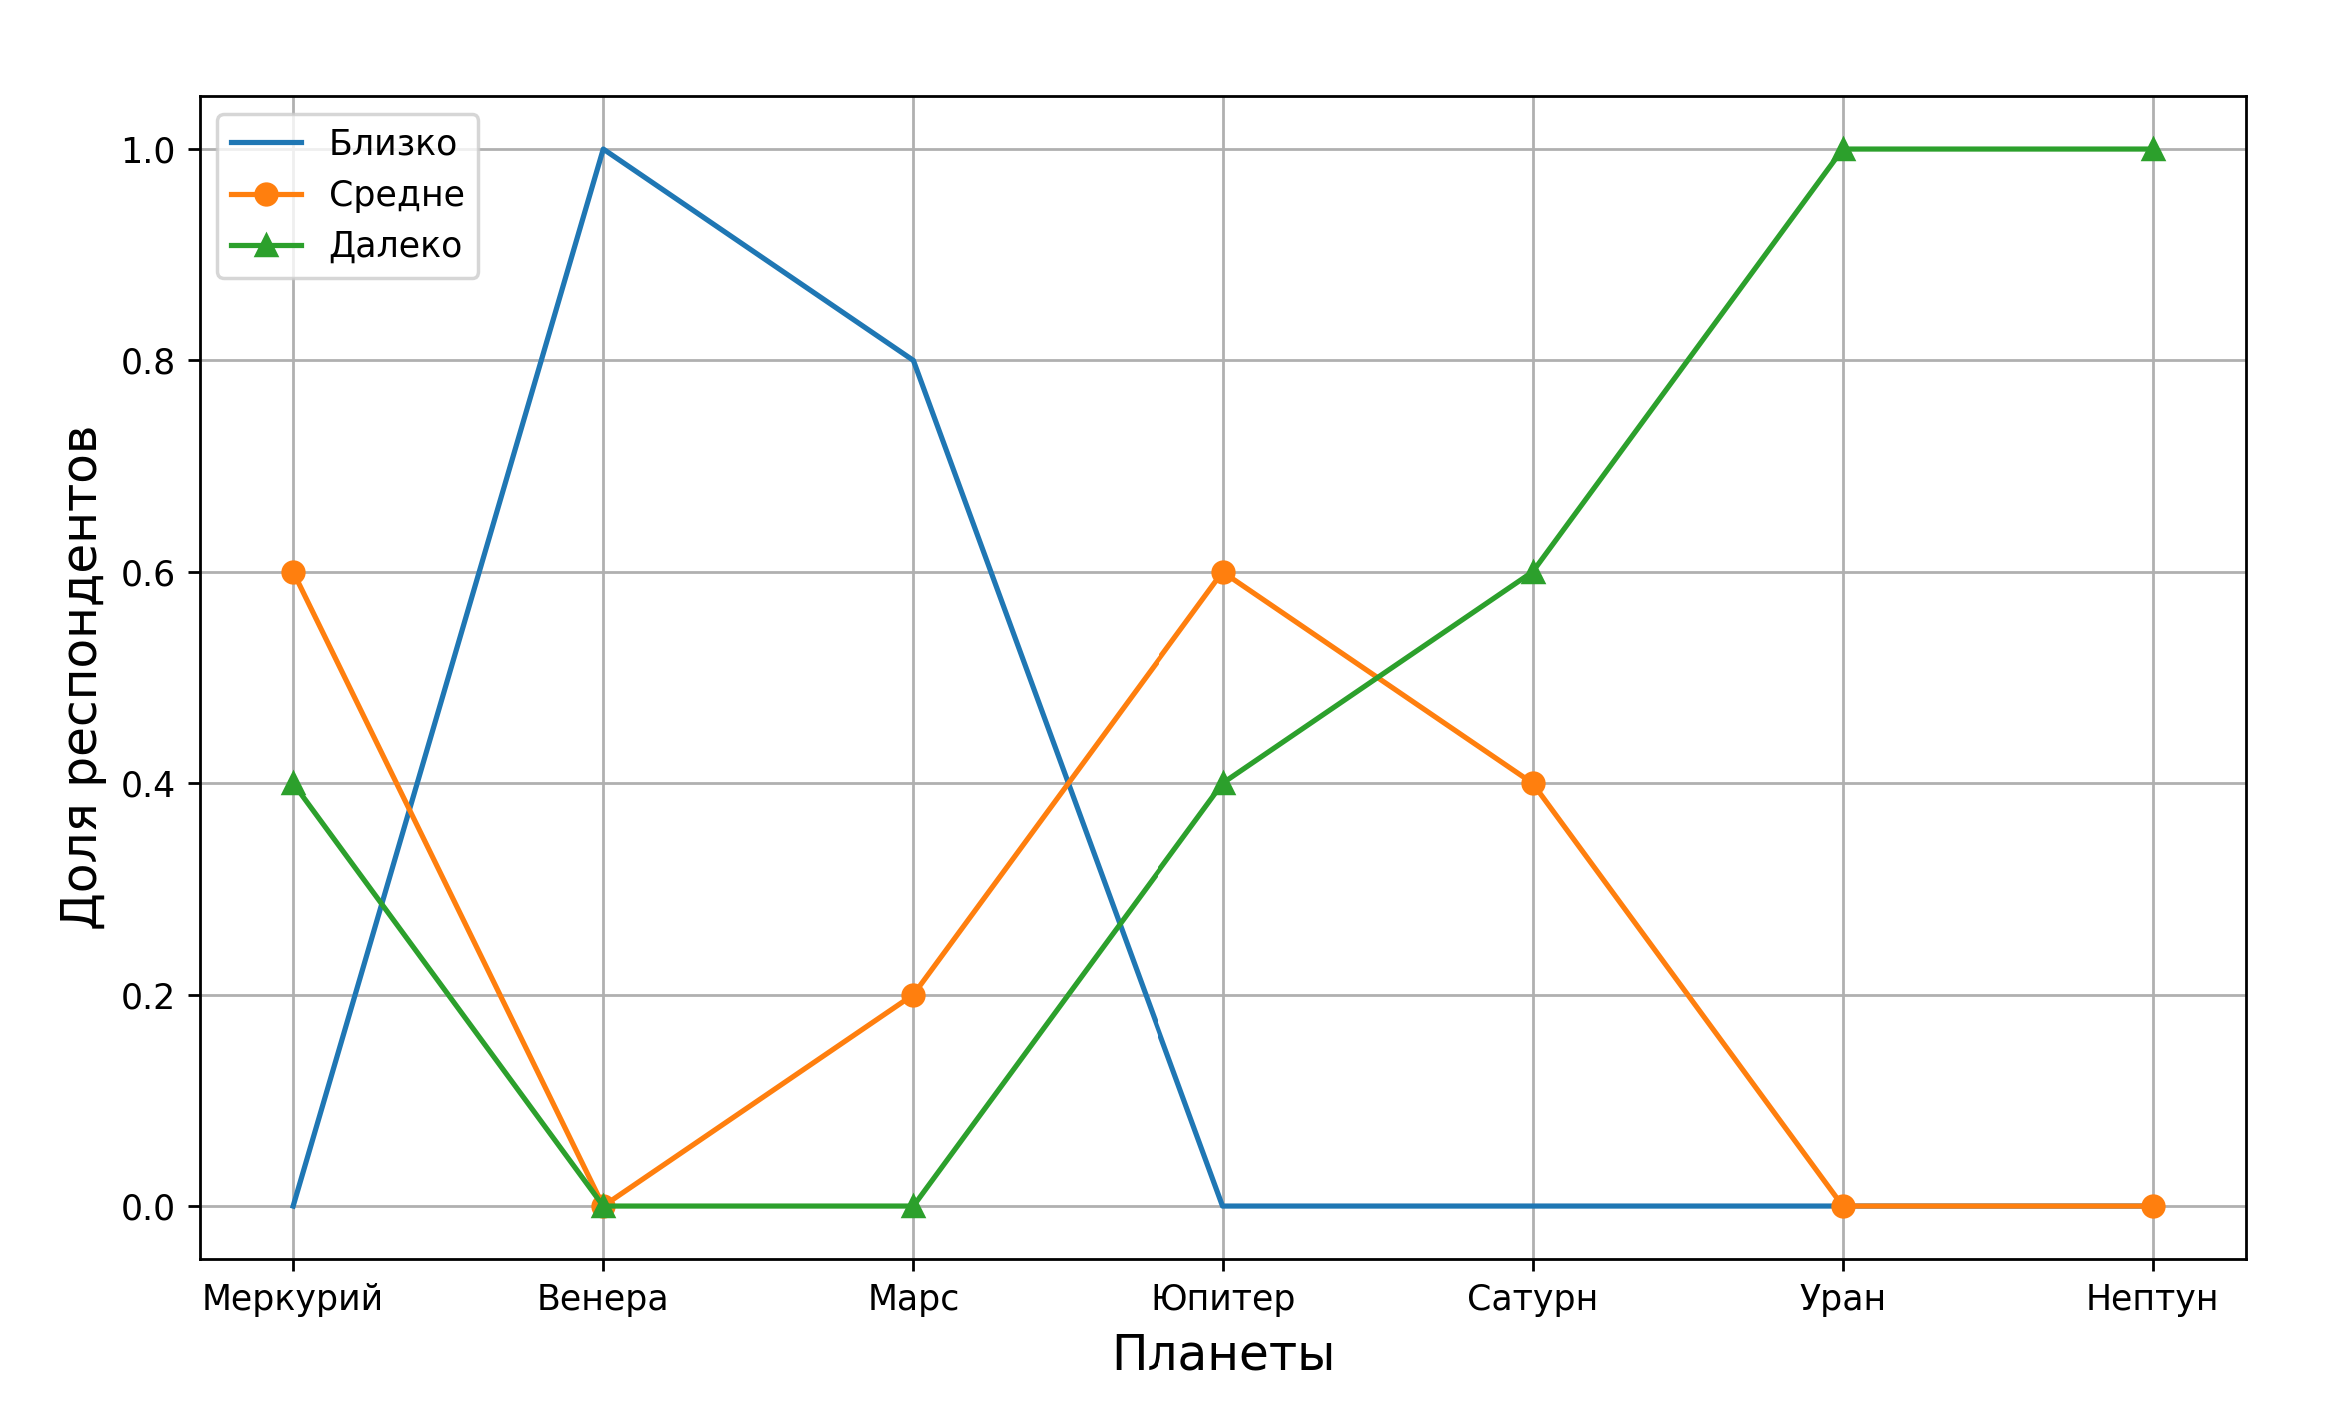
\includegraphics[width=450pt]{inc/answers.png}
	\caption{Функции принадлежности термам значений переменной}
	\label{fig:answers}	
\end{figure}

\vspace{\baselineskip}
\subsection{Демонстрация работы программы}
\vspace{\baselineskip}

На рисунке \ref{fig:output} представлен пример работы программы.
Пользователь вводит вопрос на естественном языке, программа выдает результаты в виде кортежей (<<слово>>, <<страница в словаре>>).

\begin{figure}[h!btp]
	\centering
	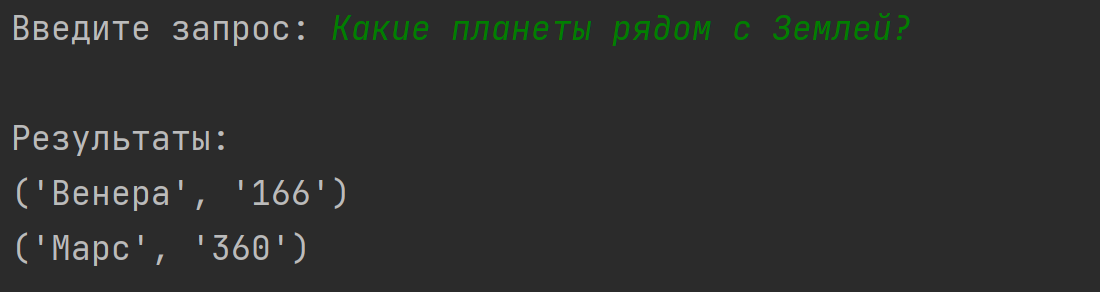
\includegraphics[width=420pt]{inc/output1.png}
	\caption{Пример работы реализаций алгоритмов}
	\label{fig:output}	
\end{figure}

\begin{figure}[h!btp]
	\centering
	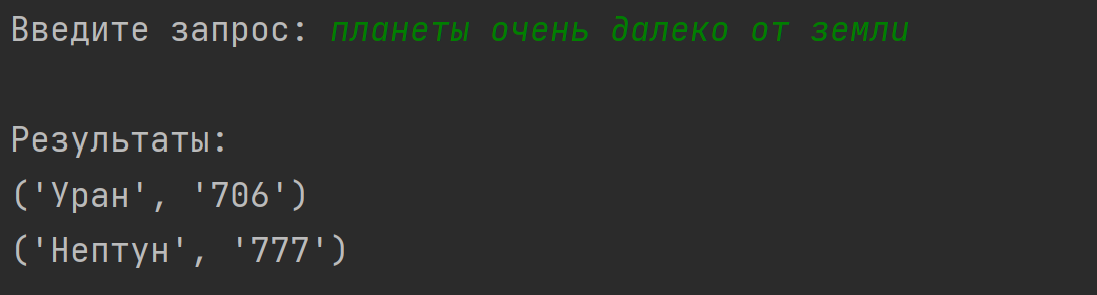
\includegraphics[width=420pt]{inc/output2.png}
	\caption{Пример работы реализаций алгоритмов}
	\label{fig:output}	
\end{figure}

\begin{figure}[h!btp]
	\centering
	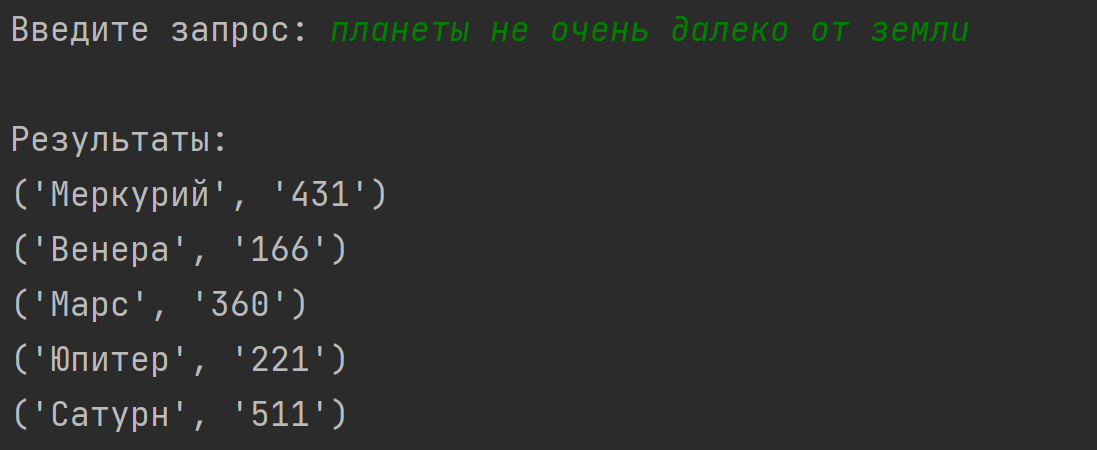
\includegraphics[width=420pt]{inc/output3.png}
	\caption{Пример работы реализаций алгоритмов}
	\label{fig:output}	
\end{figure}

\begin{figure}[h!btp]
	\centering
	
\includegraphics[width=420pt]{inc/output4.png}
	\caption{Пример работы реализаций алгоритмов}
	\label{fig:output}	
\end{figure}

\vspace{\baselineskip}
\subsection*{Вывод}
\vspace{\baselineskip}

Были приведены результаты опроса респондентов и построены графики функций принадлежности значений переменной термам. Также были рассмотрены примеры работы программы.

Разработанный метод рекомендуется к применению. Ограничением метода является соответствие круга респондентов кругу пользователей: если бы респондентами выступали астрономы, то потребовалось бы провести отдельный опрос среди соотвтетсвующей профильной выборки респондентов, что дало бы иные результаты в части диапазонов значений расстояний между небесными телами, соответствующих выбранным термам. 